% Where the cited defenses act on the path of an OTP request (manuscript Section 2).
% Build: pdflatex fig8_defense_path.tex; pdftoppm -r 220 -png -singlefile fig8_defense_path.pdf fig8_defense_path
\documentclass[tikz,border=2pt]{standalone}
\usepackage{times}
\usetikzlibrary{positioning,arrows.meta}
\begin{document}
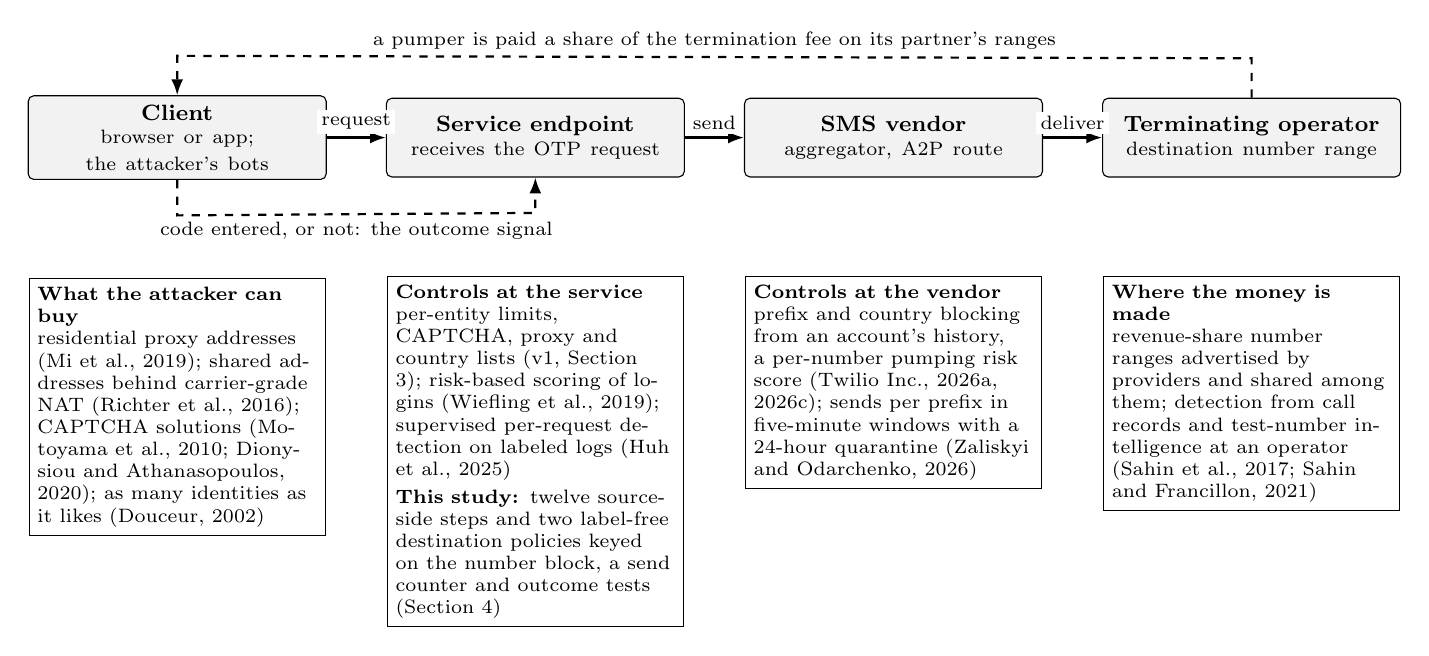
\begin{tikzpicture}[
  stage/.style={draw, rounded corners=2pt, align=center, minimum height=1.0cm, text width=3.55cm, font=\footnotesize\bfseries, fill=gray!10},
  note/.style={draw, align=left, text width=3.55cm, font=\scriptsize, inner sep=3pt, fill=white},
  arr/.style={-{Latex[length=2mm]}, thick},
  back/.style={-{Latex[length=2mm]}, thick, dashed},
  lab/.style={font=\scriptsize, fill=white, inner sep=1.5pt}
]
\node[stage] (client) {Client\\[-1pt]{\mdseries\scriptsize browser or app; the attacker's bots}};
\node[stage, right=0.75cm of client] (service) {Service endpoint\\[-1pt]{\mdseries\scriptsize receives the OTP request}};
\node[stage, right=0.75cm of service] (vendor) {SMS vendor\\[-1pt]{\mdseries\scriptsize aggregator, A2P route}};
\node[stage, right=0.75cm of vendor] (operator) {Terminating operator\\[-1pt]{\mdseries\scriptsize destination number range}};
\draw[arr] (client) -- node[lab, above=1pt]{request} (service);
\draw[arr] (service) -- node[lab, above=1pt]{send} (vendor);
\draw[arr] (vendor) -- node[lab, above=1pt]{deliver} (operator);
\draw[back] (operator.north) -- ++(0,0.5) -- node[lab, above=1pt]{a pumper is paid a share of the termination fee on its partner's ranges} ([yshift=0.5cm]client.north) -- (client.north);
\draw[back] (client.south) -- ++(0,-0.45) -- node[lab, below=1pt]{code entered, or not: the outcome signal} ([yshift=-0.45cm]service.south) -- (service.south);

\node[note, below=1.25cm of client] (nclient) {\textbf{What the attacker can buy}\\
residential proxy addresses (Mi et al., 2019); shared addresses behind carrier-grade NAT (Richter et al., 2016); CAPTCHA solutions (Motoyama et al., 2010; Dionysiou and Athanasopoulos, 2020); as many identities as it likes (Douceur, 2002)};
\node[note, below=1.25cm of service] (nservice) {\textbf{Controls at the service}\\
per-entity limits, CAPTCHA, proxy and country lists (v1, Section 3); risk-based scoring of logins (Wiefling et al., 2019); supervised per-request detection on labeled logs (Huh et al., 2025)\\[2pt]
\textbf{This study:} twelve source-side steps and two label-free destination policies keyed on the number block, a send counter and outcome tests (Section 4)};
\node[note, below=1.25cm of vendor] (nvendor) {\textbf{Controls at the vendor}\\
prefix and country blocking from an account's history, a per-number pumping risk score (Twilio Inc., 2026a, 2026c); sends per prefix in five-minute windows with a 24-hour quarantine (Zaliskyi and Odarchenko, 2026)};
\node[note, below=1.25cm of operator] (noperator) {\textbf{Where the money is made}\\
revenue-share number ranges advertised by providers and shared among them; detection from call records and test-number intelligence at an operator (Sahin et al., 2017; Sahin and Francillon, 2021)};
\end{tikzpicture}
\end{document}
